% M. S. Tsoeu (2011), University of Cape Town <mohohlo.tsoeu@uct.ac.za>

% This is a project report templace document created for EEE4022FS students at the University of Cape Town.
%
% This file should be is processed with ``pdflatex`` and might need a few modifications if a different processor is chosen.


\documentclass[a4paper,11pt]{report}

%Include packages you need to use here

\usepackage[top = 1in, bottom = 1in, left = 1in, right = 1in]{geometry}
\usepackage{graphicx}
\usepackage{fancyhdr}
\usepackage{amsmath, amsthm, amssymb}
\usepackage{lastpage}
\usepackage{subfigure}
\usepackage{lscape}
\usepackage{hyphenat}
\usepackage{setspace}
\usepackage{hyperref}
% for font
\usepackage{mathptmx}
% for code
\usepackage{listings}
\usepackage{xcolor}
% For better tables
\usepackage{array}       % for >{\raggedright\arraybackslash}p{..}
\usepackage{booktabs}    % optional, nicer horizontal rules
\usepackage{float}

\lstset{
  basicstyle=\ttfamily\small,
  keywordstyle=\color{blue},
  commentstyle=\color{gray}\itshape,
  frame=single,
  breaklines=true
}

\lstdefinelanguage{yaml}{
  basicstyle=\ttfamily\small,
  morekeywords={true,false,null},
  sensitive=false,
  comment=[l]{\#}
}

% Include page formatting here. 
\parskip = 6mm
\parindent = 0mm
\renewcommand{\headrulewidth}{0pt}
\rhead[]{\thesection}
\lhead[\thechapter]{}


\begin{document}
 
% This section formats the title page of the Report.
\thispagestyle{empty}
{\Huge \begin{center}
% Modify the line below to insert your title.
Insert your title here
\hrule 
% Modify the line below to insert your subtitle.
{\Large Insert a subtitle here (if applicable)}
\end{center}}

\vskip 5mm
\begin{center}
\- \- \- \- \- \- \- \- \- \-
\includegraphics[scale = 0.3]{uctLogo.png}
\end{center}

\vskip 5mm
\begin{center}
Presented by:\\
Mohohlo Samuel T\v soeu		% Insert your name here
\end{center}

\vskip 10mm
\begin{center}
Prepared for:\\
M. S. T\v soeu\\ 		% Insert your supervisor's name here.
Dept. of Electrical and Electronics Engineering\\University of Cape Town
\end{center}


\vskip 10mm
\begin{center}
Submitted to the Department of Electrical Engineering at the University of Cape Town in partial
fulfilment of the academic requirements for a Bachelor of Science degree in ***INSERT DEGREE
NAME HERE (Electrical Engineering; Mechatronics or Electrical and Computer Engineering)

\end{center}


\vskip 5mm
\begin{center}{\bf \today}
\end{center}

\newpage
\thispagestyle{empty}
\mbox{}
\newpage

\singlespacing
\nohyphens{
\thispagestyle{empty}
\vskip 40mm


% Please leave the declaration as it is (Standard UCT declaration).
{\Large Declaration}\\
\hrule

\vskip 10mm
\begin{enumerate}
\item I know that plagiarism is wrong. Plagiarism is to use another's work and pretend that it is one's
own.
\item I have used the IEEE convention for citation and referencing. Each contribution to, and quotation in,
this report from the work(s) of other people has been attributed, and has been cited and
referenced.
\item This report is my own work.
\item I have not allowed, and will not allow, anyone to copy my work with the intention of passing it off
as their own work or part thereof.
\end{enumerate}
\vskip 10mm
Signature:\ldots\ldots\ldots\ldots\ldots\ldots\ldots\ldots\ldots 
\\M. S. T\v soeu 		% Chante this line to your name.
\vskip10mm
Date:\ldots\ldots\ldots\ldots\ldots\ldots\ldots\ldots\ldots\ldots .

\newpage
\thispagestyle{empty}
{\Large Terms of Reference}\\
\hrule

The terms of reference page is an agreement between yourself and your supervisor outlining what is expected of you in your final year project. Please make sure that this is discussed and written at the beginning of your thesis project. 


\fancyfoot[C]{\thepage}
\pagestyle{plain}
\newpage
\pagenumbering{roman}
{\Large Acknowledgments}\\
\hrule
Make relevant acknowledgements to people who have helped you complete or conduct this work, including sponsors or research funders.


\newpage

{\Large Abstract}\\
\hrule

% Place your abstract here.
\begin{itemize}
\item Open the {\bf Project Report Template.tex} file and carefully follow the comments (starting with \%).
\item Process the file with {\bf pdflatex}, using other processors may need you to change some features such as graphics types.
\item Note the files included in the  {\bf Project Report Template.tex} (with the .tex extension excluded). You can open these files separately and modify their contents 
or create new ones.
\item Contact the latex namual for more features in your document such as equations, subfigures, footnotes, subscripts \& superscripts, special characters etc.
\item I recommend using the {\bf kile} latex IDE, as it is simple to use.
\end{itemize}


\newpage
\tableofcontents

%\newpage
%\listoffigures

%\newpage
%\listoftables

% Page formatting, to place section titles as headers of odd pages and Chapter titles as headers of even pages.
\newpage
\fancyhead[RE,LO]{}
\fancyhead[LE]{\leftmark}
\fancyhead[RO]{\rightmark}
\pagestyle{fancy}

\pagenumbering{arabic}

% THe files included below are .tex files containing the respective chapters these are already created in this package and you can add to or modify them.
\chapter{Introduction}

\section{Background to the study}
A very brief background to your area of research. Start off with a general introduction to the area and
then narrow it down to your focus area. Used to set the scene \cite{smt2011}.
\section{Objectives of this study}
\subsection{Problems to be investigated}
Description of the main questions to be investigated in this study.
\subsection{Purpose of the study}
Give the significance of investigating these problems. It must be obvious why you are doing this study
and why it is relevant.

\section{Scope and Limitations}
Scope indicates to the reader what has and has not been included in the study. Limitations tell the
reader what factors influenced the study such as sample size, time etc. It is not a section for excuses as
to why your project may or may not have worked.

\section{Plan of development}
Here you tell the reader how your report has been organised and what is included in each
chapter.

{\bf I recommend that you write this section last. You can then tailor it to your report.}

\chapter{Literature Review}

\section{ZephyrOS}

The \textbf{Zephyr Project} provides a scalable, open-source Real-Time Operating System (RTOS) engineered for resource-constrained embedded systems, from low-power IoT nodes to complex edge computing devices~\cite{source}. Governed by the \textbf{Linux Foundation}~\cite{source}, it is developed primarily for IoT applications with a strong emphasis on security, portability, and long-term support~\cite{source}.

\subsection{West}

A Zephyr project is managed using \textbf{West}, a command-line meta-tool designed to handle the multi-repository nature of the ecosystem. West creates and manages a \textit{workspace}, which is a top-level directory containing all Git repositories required for a project, including the core Zephyr RTOS, external modules, and the user's application code.

The workspace is organized around a central \textit{manifest repository}, which for a typical application is the repository containing the developer's primary source code. This repository must contain a \texttt{west.yml} file, which serves as the manifest. This file acts as a \textit{"bill of materials,"} explicitly defining all project dependencies. For each dependency, the manifest specifies the Git repository to be cloned and, critically, the exact revision (a specific commit, tag, or branch) to be used. This practice ensures that every developer on a project can create an identical and reproducible development environment.

A manifest file is structured in YAML. For example:

\begin{verbatim}
manifest:
  remotes:
    # Defines shortcuts for base URLs
    - name: zephyrproject-rtos
      url-base: https://github.com/zephyrproject-rtos
    - name: your-github-account
      url-base: https://github.com/your-name
      
  projects:
    # Defines the main Zephyr repository as a dependency
    - name: zephyr
      remote: zephyrproject-rtos
      revision: main
      path: zephyr

  self:
    # Describes this manifest's repository itself
    path: my-cool-app
\end{verbatim}

To create a new workspace from such a project, a developer uses the \texttt{west init} command, pointing it to the manifest repository. This command creates the workspace directory and clones the manifest repository itself. For a manifest located at \texttt{https://github.com/your-name/my-cool-app}, the command would be:

\begin{verbatim}
west init -m https://github.com/your-name/my-cool-app --mr main my-project-workspace
\end{verbatim}

After initialization, the developer navigates into the new directory and runs \texttt{west update}. This command reads the \texttt{west.yml} manifest that was just cloned. It then proceeds to synchronize the workspace by cloning all the other repositories listed in the \texttt{projects:} section—in this case, it would clone the main \texttt{zephyr} repository into the \texttt{zephyr/} directory. This ensures the entire workspace is in the exact state defined by the manifest.


\chapter{Setup}

% \section{Functional Objective and System Requirements}
% \label{sec:objective}
% 
% The central aim of this project is to build an intelligent, self-managing networking system for an embedded device. This system's purpose is to ensure that the device always stays connected by automatically choosing the best available network path.

% \subsection{Adaptive Network Wrapper: Core Function}
% The system's primary component is a custom network wrapper that intercepts all outbound application-level network requests. This wrapper must function as an intermediary, routing traffic through one of two configured internal network paths: a high-throughput Wi-Fi connection or a reliable GSM connection.

% \subsubsection{Design Requirements}
% The wrapper's design is driven by the following functional and architectural requirements:

% \begin{itemize}
%     \item \textbf{Route Abstraction:} The system must expose a unified $\text{API}$ (Application Programming Interface) to the application programmer that is functionally equivalent to standard socket operations (e.g., connect, send, receive). The application must remain agnostic to the underlying network interface selection or dynamic switching events.
%     \item \textbf{Interface Compatibility:} The system requires two internal network routes that are compatible with the host operating system's networking stack. In this project, the implementation is built upon the existing networking framework provided by the $\text{Zephyr RTOS}$.
%     \item \textbf{Selection Logic:} The wrapper must contain adaptive logic to select the optimal route based on configurable criteria, such as interface availability, connection stability, or pre-defined preference.
%     \item \textbf{Modular Expansion:} The architecture must be sufficiently modular to allow the future integration of additional network routes (e.g., $\text{Ethernet}$, $\text{BLE}$) with minimal modification to the core routing logic.
% \end{itemize}

% \subsection{Test Case: Firmware Over-the-Air (FOTA) Update}
% The operational success of the adaptive network wrapper will be verified using a highly demanding real-world test case: a $\text{FOTA}$ (Firmware Over-the-Air) update.

% \begin{itemize}
%     \item \textbf{Verification Criterion:} A successful $\text{FOTA}$ update requires a sustained, reliable network connection to download a new application image from a remote server.
%     \item \textbf{Functional Proof:} The update process must complete successfully even when the primary network route ($\text{Wi-Fi}$) is deliberately disabled during the download. This demonstrates the wrapper's ability to transparently failover to the $\text{GSM}$ route and maintain the session integrity required for the $\text{FOTA}$ transaction.
%     \item \textbf{Test Payload:} The update will transition the $\text{microcontroller}$ from a basic slow-blinking $\text{LED}$ application to a fast-blinking $\text{LED}$ application, providing clear visual confirmation of the successful firmware transfer and execution.
% \end{itemize}

\section{Hardware Description}
\label{sec:hardware}

The adaptive networking solution was developed and validated on a custom hardware platform integrating a host microcontroller unit (MCU) running the Zephyr RTOS and an external cellular modem responsible for network offloading.

\subsection{Microcontroller Unit}
\label{ssec:mcu}
The host MCU responsible for executing the application code is an Espressif ESP32-DOIT Development Board.

\begin{itemize}
    \item \textbf{SoC:} Espressif ESP32 dual-core Wi-Fi/Bluetooth Chip.
    \item \textbf{Role:} Serves as the main processing unit and provides the Wi-Fi hardware.
    \item \textbf{Power Requirement:} The board is powered via its Micro-USB port, requiring a nominal 5V supply. The max operating current for the host MCU (including the Wi-Fi radio) is XXX, which is easily sourced from a standard 5V power adapter or computer USB port.
    \item \textbf{Status Indicators:} The onboard LED was utilized for general application status feedback.
\end{itemize}

\subsection{Cellular Modem}
\label{ssec:modem}
The cellular modem is the SIMCom A7670G. This module is utilized to establish and manage the cellular data connection for the GSM network route.

\begin{itemize}
    \item \textbf{Module:} SIMCom A7670G.
    \item \textbf{Form Factor:} The module was mounted on a generic breakout board. Communication and control were achieved using standard AT Command protocol over a Universal Asynchronous Receiver/Transmitter (UART) interface.
    \item \textbf{Antenna:} A cellular antenna was connected to the module via a standard U.FL connector for reception and transmission.
    \item \textbf{Subscriber Identity:} A provisioned \textbf{SIM card} was required and inserted into the board's slot to establish a cellular data connection.
    \item \textbf{Status Indicators:} The module includes dedicated onboard LEDs to indicate its operational status: not powered, powered but idle, searching for network, and connected to the network.
\end{itemize}

\subsection{Inter-Module Communication}
The host ESP32 and the A7670 module were interfaced through the following pins:

\begin{table}[H]
    \centering
    \caption{Inter-Module Connection Summary}
    \label{tab:connections}
    \renewcommand{\arraystretch}{1.5}
    \begin{tabular}{>{\raggedright\arraybackslash}p{3cm} 
                    >{\raggedright\arraybackslash}p{3cm} 
                    >{\raggedright\arraybackslash}p{8cm}}
        \hline
        \textbf{ESP32 Pin} & \textbf{A7670G Pin} & \textbf{Function} \\
        \hline
        RX2 & TXD & Serial data reception on ESP32, receiving AT command responses and unsolicited data from the modem. \\
        TX2 & RXD & Serial data transmission from ESP32, used to send AT commands to the modem. \\
        GPIO4 & PEN (Power Enable) & Control pin for power cycling the modem. Pulling this pin to GND initiates a hardware reset/restart sequence. \\
        GND & GND & Establishes a common ground reference between the ESP32 and the modem for stable UART communication and power circuits. \\
        \hline
    \end{tabular}
\end{table}


\subsection{Power Supply}
\label{ssec:power}
The system requires two separate power feeds to accommodate the distinct current demands of the host microcontroller and the cellular modem.

\begin{itemize}
    \item \textbf{Host Microcontroller Power (ESP32):} The ESP32 development board is powered through its dedicated Micro-USB port using a 5V supply. The maximum current requirement for the ESP32 (when utilizing Wi-Fi) is approximately 500 mA. This low requirement means a standard computer USB port is sufficient to reliably power the host unit.

    \item \textbf{Cellular Modem Power (A7670G):} The A7670G modem requires a dedicated 5V supply capable of delivering peak currents up to 2A during cellular transmission bursts.

    \item \textbf{Decoupling Capacitance:} The modem's high instantaneous current draw poses significant power management challenges, often leading to voltage drop (commonly known as brown-out conditions) that can cause modem resets. To guarantee stability and hardware reliability, an extensive array of decoupling capacitors was implemented.

    \item \textbf{Capacitor Bank:} The design significantly exceeded the manufacturer's suggested minimum of 300 $\mu$F for voltage stability. The implemented capacitor bank utilizes:
    \begin{itemize}
        \item Two 4700$\mu$F aluminum electrolytic capacitors for bulk energy storage.
        \item Twelve 100nF ceramic capacitors for high-frequency noise suppression.
    \end{itemize}
    These components were soldered as close as possible to the modem board's VIN and GND pins. This physical proximity is critical to minimize parasitic inductance and resistance in the trace, allowing the capacitors to supply the high, sudden current peaks immediately and maintain the required stable voltage rail.
\end{itemize}

\subsection{Physical Assembly and Debugging}
\label{ssec:assembly}
The ESP32 and A7670G boards, along with the capacitors, were mounted onto a common stripboard base. Female pin headers were soldered onto the stripboard for both modules, facilitating non-permanent connections and easy rearrangement using male-to-male jumper wires. The capacitors were soldered directly with substantial solder to ensure robust, low-resistance connections. Two separate Micro-USB cables were used to power the ESP32 and the A7670G module's power circuit independently. A laptop was used to monitor logs from the ESP32 using UART for debugging the application.

\begin{figure}[H]
    \centering
    
\includegraphics[width=0.75\textwidth]{placeholder.jpg}
    \caption{Circuit diagram illustrating the physical interconnections between the ESP32, the A7670G modem, and the decoupling capacitor bank. Essential connections for UART communication and modem power control (PEN) are highlighted.}
    \label{fig:hardware-schematic}
\end{figure}

\begin{figure}[H]
    \centering
    % First minipage for the image with boards plugged in
    \begin{minipage}{0.48\textwidth} % Adjust width as needed (e.g., 0.48 for slight gap)
        \centering
        
\includegraphics[width=\linewidth]{placeholder.jpg} % Replace with actual filename
        \caption{Final hardware assembly showing the ESP32 (left) and A7670G (right) modules with the jumper connections between them.}
        \label{fig:hardware-photo-modules}
    \end{minipage}
    \hfill % This command adds horizontal space, pushing minipages apart
    % Second minipage for the image showing capacitors
    \begin{minipage}{0.48\textwidth} % Same width as the first
        \centering
        
\includegraphics[width=\linewidth]{placeholder.jpg} % Replace with actual filename
        \caption{Underlying stripboard assembly with modules removed showing the capacitors close to the power pins of the A7670G board.}
        \label{fig:hardware-photo-caps}
    \end{minipage}
\end{figure}

\section{Development Environment}

\subsection{Justification for Using Podman}

For this project, the primary requirement is a simple, efficient, and effective tool to create an isolated environment that ensures reproducible results. After evaluating traditional Virtual Machines (VMs), Docker, and Podman, we selected Podman as the most suitable solution. Its core advantage is providing the necessary environment isolation for reproducibility without the overhead of full virtualization or the architectural complexities of a daemon-based container engine.

Traditional VMs offer the highest level of isolation by virtualizing an entire hardware stack and running a full guest operating system. While this guarantees a completely separate environment, it comes at a significant cost in terms of performance, disk space, and startup time~\cite{ibm_containers_vs_vms}. For this project, which focuses on application-level reproducibility, such heavy-handed isolation is unnecessary and counterproductive.

Both Docker and Podman provide lightweight OS-level virtualization (containerization), which is better suited to our needs. They offer nearly identical interfaces, packaging an application and its dependencies into a container that runs on the host operating system's kernel. However, a key architectural difference makes Podman the simpler and more secure choice. Docker relies on a continuously running background daemon process (\texttt{dockerd}) with root privileges, introducing a single point of failure and potential security concerns~\cite{docker_overview, podman_overview}.

In contrast, Podman employs a daemonless architecture~\cite{podman_overview}, running containers as child processes of the user's login session and eliminating the need for a persistent, privileged background service.

While both Docker and Podman meet the project’s requirements, Podman’s simpler and more secure design makes it the preferred choice. The entire development and build workflow for this project is executed within a Podman container. See [provide instructions or appendix] for detailed container setup and configuration.

\section{Containerized Workspace Setup}

To guarantee a consistent and reproducible build environment, the entire project workspace is constructed within a Podman container. This process is automated by a Containerfile that begins with a clean Ubuntu base image and systematically installs all necessary dependencies.

The setup procedure involves several key steps. First, essential system packages such as python3, pip, venv, and git are installed. Following the installation of dependencies, a Python virtual environment is created to ensure that the west tool and its own dependencies are isolated from the system's Python installation. Once the virtual environment is activated, west is installed using pip.

With the build tools in place, the project workspace is initialized. The west init command is executed, pointing to the project's manifest repository. This is followed by west update, which reads the manifest file and clones the Zephyr source code and all other required modules, such as hal\_espressif and mcuboot, into the workspace. The complete Containerfile that encapsulates this entire setup process is detailed below.

A final manual configuration step is required to link the workspace with the Zephyr build system. After the \texttt{west update} command completes, the local west configuration file, located at \texttt{EEE4022S-Workspace/.west/config}, must be modified. The following lines need to be appended to this file:

\begin{verbatim}
[zephyr]
base = zephyr
\end{verbatim}

This configuration explicitly tells the \texttt{west} tool that the \texttt{zephyr} directory, cloned as a project dependency, is the Zephyr base to be used for all subsequent build and flash commands. With this setting in place, the workspace is fully configured and ready for firmware development.

\subsection{Project Directory Structure}

The project's directory structure is intentionally modeled after the official Zephyr \texttt{example-application} repository, which represents a best-practice approach for creating scalable and maintainable freestanding applications. This structure is designed to cleanly separate application code, custom drivers, and dependency management.

The key organizational principles adopted are as follows:

\begin{enumerate}
    \item \textbf{Multi-Application Support:} The root of the repository, which serves as the \texttt{west} manifest, is designed to house multiple distinct firmware targets. Each application is contained within its own directory, prefixed with \texttt{app-} (e.g., \texttt{app-fota-client}). This convention allows for different applications to coexist within a single version-controlled project while sharing common modules and drivers.

    \item \textbf{Custom Driver Organization:} All custom, out-of-tree drivers are consolidated under a top-level \texttt{drivers/} directory. This separates hardware-specific implementation details, such as the driver for the \texttt{simcom-a76xx} modem, from the main application logic. This modular approach promotes code reuse and simplifies maintenance, as the driver code is not tightly coupled with any single application.

    \item \textbf{Public API Headers:} A corresponding \texttt{include/} directory is used to store the public header files for the custom drivers. This follows standard software engineering practices, creating a clear distinction between the driver's public API (the functions an application can call) and its private implementation.
\end{enumerate}

Adhering to this established structure ensures that the project remains organized, scalable, and easy for other developers familiar with the Zephyr ecosystem to navigate.

\subsection{CMakeLists.txt Structure and Rationale}

The project's build system is organized using a hierarchical set of \texttt{CMakeLists.txt} files. At the top level, the main \texttt{CMakeLists.txt} sets up project-wide configurations and include directories:

\begin{verbatim}
zephyr_syscall_include_directories(include)
zephyr_include_directories(include)

add_subdirectory(drivers)
add_subdirectory(lib)
\end{verbatim}

The commands \texttt{zephyr\_syscall\_include\_directories()} and \texttt{zephyr\_include\_directories()} establish the paths to header files needed throughout the project. Unlike standard CMake projects, most CMake commands here are not the vanilla CMake commands; instead, Zephyr provides wrapper commands, all prefixed with \texttt{zephyr\_}, which encapsulate project-specific behavior and best practices. These lines are largely boilerplate for setting up the Zephyr build environment.

The most important aspect of this setup is the use of \texttt{add\_subdirectory(...)}, which defines a hierarchical chain of build configurations. When a subdirectory is added, its own \texttt{CMakeLists.txt} is processed in the context of the parent, inheriting global settings while allowing subdirectory-specific configuration. This means that any configuration in a given \texttt{CMakeLists.txt} applies to the files in that directory and all of its descendants, creating a structured and modular build process.

To avoid unnecessary compilation, environment variables can specify which modules should be included in the build. This is largely managed through \texttt{Kconfig}, as described in Section XXX. Zephyr provides the command \texttt{add\_subdirectory\_ifdef(Variable directory-name)} to conditionally add a subdirectory only if a corresponding configuration variable is enabled.

CMake operates at a higher level of abstraction than directly invoking the compiler. It specifies what to build and how components relate to one another, leaving the actual compilation commands to the underlying build system. In the case of Zephyr, the CMake configuration is ultimately converted into \texttt{ninja} build files, which handle the low-level compilation of the application.

Other CMake commands in the project serve similar organizational or configuration purposes and can generally be considered boilerplate for setting up the Zephyr build environment. The key takeaway is that the hierarchical structure defined by \texttt{add\_subdirectory(...)}—combined with conditional inclusion—enables modular, maintainable, and scalable builds.

In addition to the module-level \texttt{CMakeLists.txt} files, each specific application in the project has its own \texttt{CMakeLists.txt}. These files typically start with:

\begin{verbatim}
cmake_minimum_required(VERSION 3.13.1)
find_package(Zephyr REQUIRED HINTS $ENV{ZEPHYR_BASE})

project(app LANGUAGES C)

target_sources(app PRIVATE src/main.c)
\end{verbatim}

Unlike the module-level files, these app-specific \texttt{CMakeLists.txt} describe exactly which source files are needed to compile the application and may specify additional files to include or compile that are not already handled by the hierarchical module chain. In essence, they define the entry point and composition of a specific app while still inheriting global configurations and include paths from the parent CMakeLists.txt files.


\section{Developing a Custom Modem Driver}

\subsection{Limitations of The Existing Driver}
While the Zephyr RTOS provides a generic cellular driver (\texttt{modem\_cellular}), it was determined to be a suboptimal choice for this project for several key reasons, necessitating the development of a custom, device-specific driver for the Simcom A7670 modem.

\begin{itemize}
    \item \textbf{Inefficiency:} The generic driver is based on an onboard networking model, utilizing the Point-to-Point Protocol (PPP). This architecture forces the host microcontroller (the ESP32) to run Zephyr's entire native TCP/IP stack. For a resource-constrained embedded system, the significant CPU and RAM overhead required to manage sockets, construct packets, and handle protocols like DNS and DHCP was deemed unacceptable, especially for a project requiring a lightweight solution.
    
    \item \textbf{Application-Specific Requirements:} The primary goal of this project is to integrate with the UpdateHub firmware-over-the-air (FOTA) platform, which operates over CoAP. While the generic driver could provide basic IP connectivity, implementing the CoAP client functionality would be more efficient by leveraging the modem's internal networking stack rather than consuming host resources. A minimal, custom driver provides the direct control needed for this specific application.

    \item \textbf{Hardware Mismatch:} The generic driver assumes a standard power-on procedure. The A7670, however, has specific timing requirements. A custom driver allowed for the implementation of a robust \texttt{modem\_autobaud} function that actively probes the modem until it confirms responsiveness. This is a far more reliable startup method than the simple timed delays assumed by a generic implementation, and complexity was further reduced by fixing the baud rate at 115200.
\end{itemize}

\subsection{Architectural Approach: Offloaded Networking}
To address the limitations of the generic driver, this project adopted the \textit{socket offload} architecture. In this model, the modem is treated as a "smart co-processor" that contains its own powerful, built-in TCP/IP stack capable of handling both TCP and UDP connections.

The responsibility of the host MCU is significantly reduced. Instead of constructing raw IP packets, the MCU's driver sends high-level, text-based commands over a UART interface, such as \texttt{AT+CIPOPEN} to request the use of a socket, followed by \texttt{AT+CIPSEND} to send data to a specific destination. The modem itself handles all the low-level complexities of the network connection, including session management and packetization. This \textit{offloads} the networking workload from the MCU, freeing up its resources for the primary application logic and resulting in a more efficient and responsive system.

% \begin{figure}[h]
%     \centering
%     % You can create a simple diagram for this and uncomment this section.
%     % \includegraphics[width=0.8\textwidth]{placeholder_diagram.png}
%     \caption{Architectural comparison of Onboard vs. Offloaded Networking.}
%     \label{fig:offload_arch}
% \end{figure}

\subsection{Implementation Language: The AT Command Set}
The primary method for controlling a cellular modem and implementing a socket offload driver is through the AT command set. Originally developed by Hayes in the 1980s, the "ATtention" command set is a human-readable, text-based language sent over a serial interface. While the basic structure is standardized, the specific commands for advanced features like TCP/IP networking can vary significantly between modem families. The A7670 modem follows the AT command set of the A76xx series, which is distinct from other Simcom modems like the SIM7080, necessitating a careful translation and adaptation of the driver logic.


Commands follow a standard structure:
\begin{itemize}
    \item \textbf{Prefix:} All commands begin with the prefix \texttt{AT}.
    \item \textbf{Command:} A specific command, often starting with \texttt{+} for extended commands (e.g., \texttt{AT+CSQ} for signal quality).
    \item \textbf{Action Suffix:}
    \begin{itemize}
        \item \texttt{?} (Read): Queries the current value of a parameter (e.g., \texttt{AT+CREG?}).
        \item \texttt{=} (Set): Sets a new value for a parameter (e.g., \texttt{AT+COPS=0}).
        \item \texttt{=?} (Test): Asks the modem to list all supported values for a parameter.
    \end{itemize}
\end{itemize}
This command-and-response protocol forms the fundamental language the driver must speak to manage the modem's state and operations.

\subsection{Modem Communication Patterns}
A robust driver must be architected to handle several distinct types of modem responses, each with its own timing and purpose.

\begin{itemize}
    \item \textbf{Solicited vs. Unsolicited Responses:} This is the most critical distinction. A \textit{solicited} response is a direct answer to a command just sent (e.g., \texttt{+CSQ: 23,0} in reply to \texttt{AT+CSQ?}). In contrast, an \textit{Unsolicited Result Code (URC)} is a message the modem sends on its own initiative to notify the host of an external event, such as an incoming call (\texttt{RING}) or a network connection being established (\texttt{+CGEV: ME PDN ACT 1}). A driver must have a background process constantly listening for URCs to accurately track the modem's state.

    \item \textbf{Response Types:}
    \begin{itemize}
        \item \textbf{Final Result Codes:} Every command execution concludes with a final code, typically \texttt{OK} for success or \texttt{ERROR} for failure. The driver must block and wait for this code to confirm a synchronous command has finished.
        \item \textbf{Intermediate Responses:} These are data-bearing responses that arrive \textit{before} the final \texttt{OK} or \texttt{ERROR}.
        \item \textbf{Data Input Prompt (\texttt{>}):} This is a special response. For commands like \texttt{AT+CIPSEND}, the modem replies with a single \texttt{>} character to signal that it is now in "data input mode" and is ready to receive the raw data payload from the host. The driver must handle this state separately from normal command responses.
    \end{itemize}
\end{itemize}


\section{Porting the SIM7080 Driver for the A7670 Modem}

The core of this project involved adapting an existing Zephyr RTOS driver for the Simcom SIM7080 modem to create a new, custom socket offload driver for the Simcom A7670. While both modems are from the same manufacturer, their hardware behavior and AT command sets have critical differences. This section details the initial phase of the porting process, focusing on the integration with the Zephyr build system.

\subsection{Phase 1: Build System Integration and Initial Scaffolding}
The first step was to establish the basic structure of the new driver within the Zephyr build environment. This involved creating the necessary `Kconfig` and `CMakeLists.txt` files to ensure the driver could be correctly configured and compiled as part of a Zephyr application. The existing SIM7080 driver was used as a template for this process.

\subsubsection{Kconfig Integration}
The Kconfig system allows a driver to be conditionally included in a project build via configuration flags set in the `prj.conf` file. A new `Kconfig` file was created for the A7670 driver by copying the file from the SIM7080 driver and performing a "find and replace" on all relevant identifiers. Key changes included:

\begin{itemize}
    \item Renaming the main configuration symbol from \texttt{CONFIG\_MODEM\_SIM7080} to \texttt{CONFIG\_MODEM\_A76XX}.
    \item Updating all descriptive text and help messages to refer to the A76XX series.
    \item Ensuring all dependencies on other Zephyr subsystems (such as \texttt{NETWORKING} and \texttt{GPIO}) were preserved.
\end{itemize}

This process successfully created the necessary configuration symbols to control the driver's compilation and define its dependencies within the Zephyr ecosystem.

\subsubsection{CMake Build Configuration}
The `CMakeLists.txt` file is responsible for defining which source files are compiled and what include paths are available to them. The initial configuration conditionally compiled the new `simcom-a76xx.c` driver file based on the Kconfig symbols:

\begin{verbatim}
if (CONFIG_MODEM AND CONFIG_MODEM_A76XX)
    ...
endif()
\end{verbatim}

A significant challenge emerged during this phase. The driver relies heavily on internal "helper" components from the Zephyr modem subsystem, such as \texttt{modem\_context.h}, \texttt{modem\_cmd\_handler.h}, and \texttt{modem\_socket.h}. These headers are not part of Zephyr's public API and are therefore not exposed in the global include paths. To resolve this, a pragmatic workaround was implemented: the internal Zephyr include paths were explicitly added to the driver's compilation scope using \texttt{zephyr\_library\_include\_directories}.

\begin{verbatim}
if (CONFIG_MODEM_A76XX)
    zephyr_library_sources(simcom-a76xx.c)
    
    # Add driver's own public include directory
    zephyr_library_include_directories(../../../include)
    
    # Add internal Zephyr paths needed by the driver
    zephyr_library_include_directories(${ZEPHYR_BASE}/drivers/modem)
    zephyr_library_include_directories(${ZEPHYR_BASE}/subsys/net/ip)
    zephyr_library_include_directories(${ZEPHYR_BASE}/subsys/net/lib/sockets)
endif()
\end{verbatim}

A further complication arose because the main application (\texttt{main.c}) needs to call the public API functions of the driver (e.g., \texttt{mdm\_a76xx\_power\_on()}). The driver's public header file, \texttt{simcom-a76xx.h}, exposes data types that depend on the same internal Zephyr headers. This created a visibility issue: while the driver itself could now see the internal headers, the main application could not, leading to compilation errors. To resolve this, the same internal include paths were also added to the \texttt{CMakeLists.txt} of the main application. While this creates a tight coupling between the application and the internal structure of the Zephyr kernel, it was a necessary and effective workaround to achieve a functional build.

\subsection{Phase 2: Driver Logic and AT Command Translation}
Following the initial structural port, the core technical challenge was to adapt the driver's logic to the specific behavior and command set of the A7670 modem. This was a systematic process that involved analyzing the existing driver, consulting the A76XX Series AT Command Manual, and implementing the necessary changes.

\subsubsection{Leveraging the Zephyr Modem Subsystem}
A foundational step was to understand the abstractions provided by the Zephyr modem subsystem to avoid "reinventing the wheel." The SIM7080 driver was built upon a set of powerful but non-public helper components. An analysis of these components revealed a robust framework for handling modem interactions, which was adopted for the new driver:
\begin{itemize}
    \item \textbf{The Command Handler (\texttt{modem\_cmd\_handler}):} This component provides the core engine for parsing incoming data from the modem. It can match solicited responses and Unsolicited Result Codes (URCs) against a list of pre-defined handlers, automatically splitting responses into arguments and dispatching them to the correct C function.
    \item \textbf{The Socket Abstraction (\texttt{modem\_socket}):} This layer provides a generic way to manage the modem's internal connection "slots" (e.g., Link Numbers 0-9) and map them to standard Zephyr file descriptors, simplifying the implementation of the socket offload API.
    \item \textbf{The Synchronous Send Function (\texttt{modem\_cmd\_send}):} This helper function encapsulates the logic of sending a command, blocking on a semaphore, and waiting for a final \texttt{OK} or \texttt{ERROR} response, complete with a timeout. This greatly simplified the implementation of synchronous command-response sequences.
\end{itemize}
By reusing this existing framework, the porting effort could focus on the unique aspects of the A7670 rather than on low-level parsing and state management.

\subsubsection{The AT Command Translation Process}
The most intensive part of the porting effort was the translation of the AT command set. The process for each functional block (e.g., network activation, socket connection) was as follows:
\begin{enumerate}
    \item \textbf{Analyze High-Level Goal:} The purpose of the original AT command in the SIM7080 driver was identified. For example, the goal of \texttt{AT+CNACT=0,1} was to "activate the PDP context."
    \item \textbf{Consult A76XX Manual:} The official A76XX Series AT Command Manual was searched for the equivalent command.
    \item \textbf{Implement and Adapt:} The C code was modified to reflect the differences in the new command's syntax, parameters, and response patterns.
\end{enumerate}

This process often revealed significant differences that required more than a simple string replacement. For example, a direct translation was possible for activating the PDP context, which changed from \texttt{AT+CNACT=0,1} on the SIM7080 to \texttt{AT+CGACT=1,1} on the A7670. However, a more complex adaptation was required for the socket connection commands, which changed from the \texttt{AT+CA*} family to the \texttt{AT+CIP*} family, necessitating a complete rewrite of the socket offload functions and their associated response handlers.

\chapter{System Architecture}

\section{Hardware System Architecture}
\label{sec:hardware_architecture}

The system architecture is built upon an embedded platform comprising three main components: the ESP32 microcontroller unit, an external A7670G cellular modem and a host PC. This design defines the functional relationships among these hardware components.

The complete system's functional links, including power and communication pathways, are summarized in Table \ref{tab:arch_links} for clarity.

\begin{table}[H]
    \centering
    \caption{Summary of Functional Links and Communication Protocols}
    \label{tab:arch_links}
    \renewcommand{\arraystretch}{1.2}
    \begin{tabular}{>{\raggedright\arraybackslash}p{4cm} 
                    >{\raggedright\arraybackslash}p{2cm} 
                    >{\raggedright\arraybackslash}p{6.5cm}}
        \hline
        Functional Link & Protocol/Type & Purpose and Signals Transferred \\
        \hline
        Host PC $\rightarrow$ ESP32 & UART & Shell Commands: Input from the user (via terminal) to the ESP32 for interactive control and testing. \\
        \hline
        ESP32 $\rightarrow$ Host PC & UART & Console Output: Output stream carrying debug, kernel, and application status messages for monitoring. \\
        \hline
        ESP32 $\rightarrow$ A7670G & UART & AT Commands (Control): The host MPU sends high-level commands to control the modem's internal TCP/IP stack (e.g., connect, configuration). \\
        \hline
        A7670G $\rightarrow$ ESP32 & UART & AT Responses, URCs (Feedback): Returns the modem's feedback (OK, ERROR), Unsolicited Response Codes (URCs), and the received IP Data Payload. \\
        \hline
        ESP32 $\rightarrow$ A7670G & GPIO & PEN Control: Dedicated control line used to programmatically assert a hardware reset on the A7670G modem. \\
        \hline
        ESP32 Power Supply $\rightarrow$ ESP32 & DC Supply & 5V DC Supply: Provides operational power for the host MPU and its integrated Wi-Fi module. \\
        \hline
        A7670G Power Supply $\rightarrow$ A7670G & DC Supply & 5V DC Supply (2A Peak): High-capacity power line required to maintain voltage stability during the modem's high-current GSM transmission bursts. \\
        \hline
    \end{tabular}
\end{table} 

\begin{figure}[H]
    \centering
    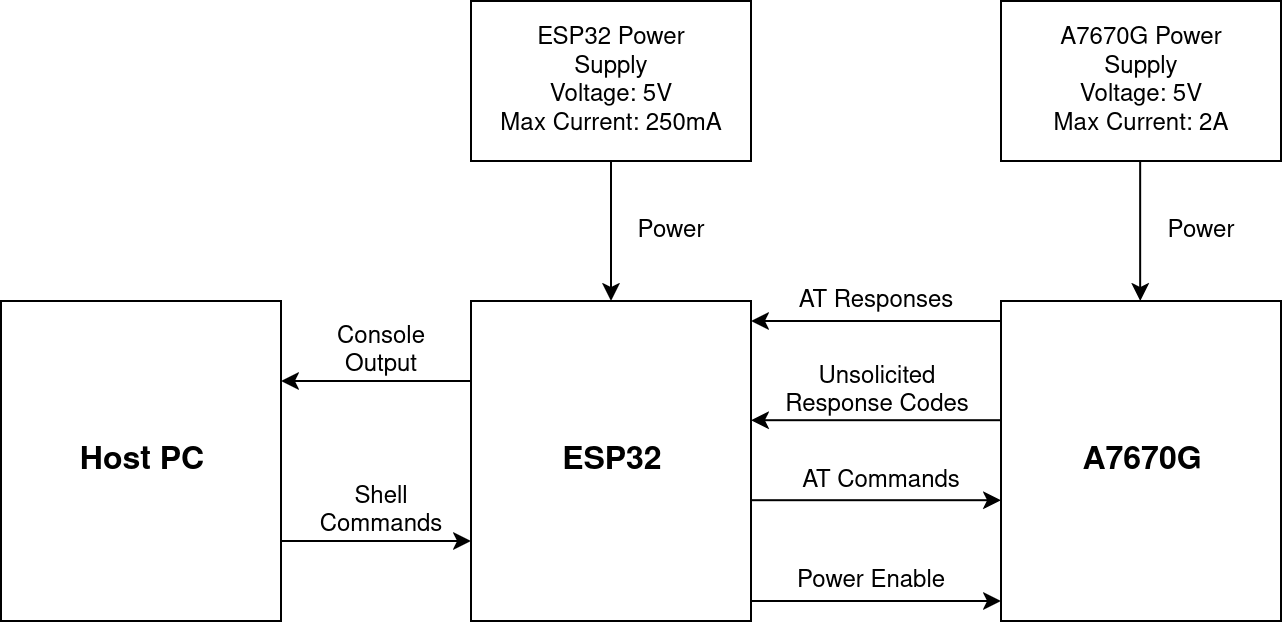
\includegraphics[width=0.85\textwidth]{"images/hardware-architecture.png"}
    \caption{Conceptual Hardware System Block Diagram. The figure illustrates the external connections and the functional relationship between the host ESP32 MPU and the external A7670G cellular modem.}
    \label{fig:hardware-arch-diagram}
\end{figure}

\section{Software Architecture}
\label{sec:software_architecture}

The software architecture is defined by the strategic layering of custom and native components within the \text{Zephyr RTOS}. The core innovation is the Adaptive Sockets Layer, designed to provide a single, resilient networking interface to the application by dynamically managing two fundamentally different network paths.

\subsection{Background: Key Zephyr Networking Abstractions}
\label{ssec:background_zephyr}

The project relies on specific networking abstractions provided by the Zephyr RTOS. Understanding the roles of these core components and the available networking paradigms is essential for interpreting the architectural diagrams:

\begin{itemize}
    \item \textbf{Sockets API:} This is the highest software layer, providing the standard POSIX-like functions (\texttt{connect}, \texttt{send}, \texttt{recv}, ...) used by application code to request network services.
    \item \textbf{Network Context (\texttt{net\_context}):} This data structure represents the state of a single network session (e.g., a TCP connection). In the native networking stack, every socket created by the application is assigned a unique Network Context.
    \item \textbf{Network Interface (\texttt{net\_if}):} A logical structure that represents a path to a specific network medium. Each physical network device has only one \texttt{net\_if} allocated at compile time.
\end{itemize}

\subsubsection{Data Handling in the Native Zephyr Stack}
When the Sockets API receives application data, it passes that data, along with the session's Network Context, to the lower layers. The data is handled by the \texttt{net\_if} for protocol processing. The Zephyr stack then performs the necessary protocol work—such as adding IP and TCP headers—before handing the network packet off to the Device Drivers, which transmit the data to the physical hardware. While the \texttt{net\_if} structure is created at compile time, network contexts are created during runtime and bound to network interfaces.

\subsection{Zephyr Networking Implementation Paradigms}
\label{ssec:networking_paradigms}
Zephyr offers flexibility in networking implementation, allowing developers to choose which protocol layers are handled by the microprocessor versus which are delegated (offloaded).

\begin{enumerate}
    \item \textbf{Native Full Stack Implementation (Standard):} The developer implements the low-level Device Driver to communicate with the L2 (Data Link) Layer. This provides very little control to the developer but allows Zephyr to automatically handle the full stack, including TCP/IP and the Sockets API. This is the path used by the Wi-Fi interface.
    \item \textbf{Network Offloading (Partial Control):} The developer implements a driver that presents a specific API used by the \texttt{net\_if}. This implementation allows the driver to bypass the L2 layer of \text{Zephyr's} native networking stack. This provides increased control over the network path but still relies on Zephyr for the higher layers (Net Contexts and Sockets).
    \item \textbf{Sockets Offloading (Full Control):} The developer implements the Sockets API and all layers below. This method provides the greatest degree of control over network behavior—a necessity for implementing dynamic routing—but makes the developer responsible for the full stack. This paradigm is typically used to integrate external hardware that executes the entire TCP/IP and Sockets stack internally. The Adaptive Sockets Layer is built atop this framework specifically to leverage this full control aspect for implementing transparent failover.
\end{enumerate}

\subsection{Software Architecture: Layer-by-Layer Implementation}
\label{ssec:software_implementation}

The architecture is built on a custom separation of management and session-handling logic. For definitions of the fundamental Zephyr networking terms used below (e.g., Network Context and $\texttt{net\_if}$), please refer to Section \ref{ssec:background_zephyr}. The structure is best understood by examining the system layer by layer, as illustrated in Figure \ref{fig:software-arch}.

\begin{figure}[H]
    \centering
    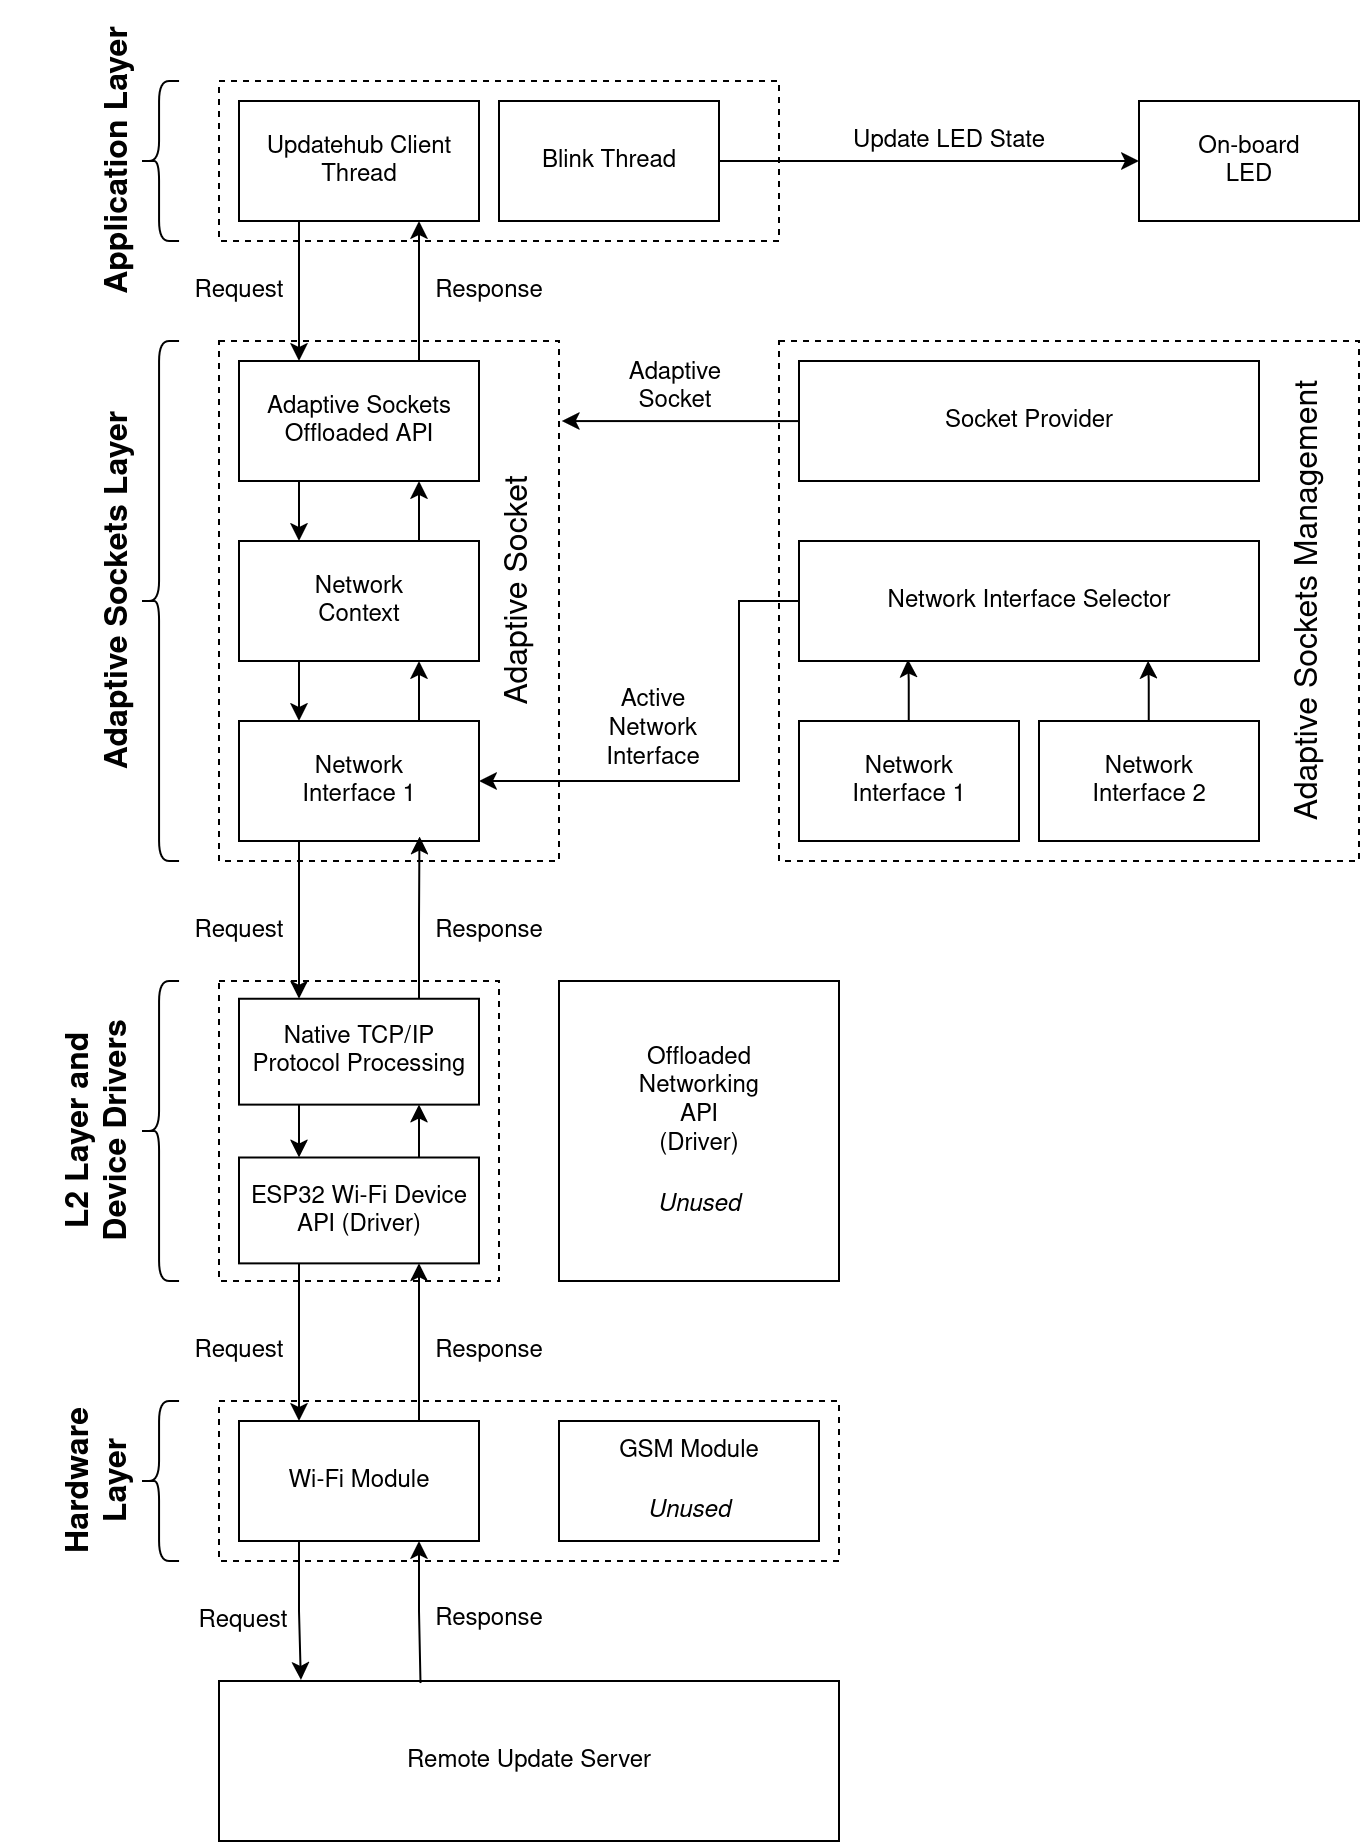
\includegraphics[width=0.95\textwidth]{"images/software-architecture.png"}
    \caption{Conceptual Software Architecture illustrating the data path of a single Adaptive Socket Instance. The diagram highlights the functional split between the Native Wi-Fi and Offloaded GSM network stacks.}
    \label{fig:software-arch}
\end{figure}

\subsubsection{Layer 1: Application Layer}
\label{sssec:application_layer}

The Application Layer sits at the highest level and contains the primary application threads that interact with the system. While the \text{Zephyr RTOS} manages numerous internal system threads for kernel operations, the following are the primary threads created and managed by the application:

\begin{itemize}
    \item \textbf{UpdateHub Client Thread:} The main application thread, which polls the \text{FOTA} server by making \textbf{Sockets API Calls} (e.g., \texttt{connect}, \texttt{send}, ...). This thread is responsible for initiating all network transactions.
    \item \textbf{Blink LED Thread:} A non-networking thread providing visual confirmation of system activity. Its blinking frequency is utilized to communicate system state: the frequency will change from a slow, steady rate to a rapid rate to confirm that a FOTA update has occurred successfully.
\end{itemize}

\subsubsection{Layer 2: Adaptive Sockets Layer (Custom Abstraction)}
\label{sssec:adaptive_sockets_layer}

The Adaptive Sockets Layer is the core innovation, providing a flexible and resilient Sockets API to the application. It is designed to be well decoupled from the physical network technologies, though for this project, it manages the Wi-Fi interface as the primary link and the GSM interface as the secondary. This layer is split into two primary functional components:

\paragraph{Adaptive Socket (The Router)}
This is the session-specific structure returned to the application. The primary logic to switch networks is embedded within the socket itself, allowing it to perform dynamic failover checks on every operation.

\begin{itemize}
    \item \textbf{Adaptive Sockets Offloaded API:} The API entry point for the session. Because the Adaptive Sockets implementation is registered as the highest priority sockets API provider in Zephyr, the operating system routes the application's generic Sockets API Calls directly to the Adaptive Sockets Layer.
    \item \textbf{Network Context:} The singular session state data structure. It is contained within the socket instance and is the element that gets re-bound to a different $\texttt{net\_if}$ during failover.
    \item \textbf{Network Interface Reference ($\texttt{net\_if}$):} A pointer to the currently assigned Network Interface (Wi-Fi or GSM).
\end{itemize}

\paragraph{Adaptive Sockets Management (The Manager)}
The Layer acts as the central policy manager and resource provider, holding the following helpers and resources:

\begin{itemize}
    \item \textbf{Network Interface References ($\texttt{net\_if\_1}$ and $\texttt{net\_if\_2}$):} Holds static references to the two possible network interfaces.
    \item \textbf{Operational Status Fields:} Internal flags updated by the Monitoring Thread that track the current viability and stability of the underlying network links.
    \item \textbf{Network Interface Selector (Helper):} A helper function that reads the $\text{Operational Status Fields}$ to determine the optimal $\texttt{net\_if}$ reference at a given moment (e.g., for initial setup).
    \item \textbf{Socket Factory (Provider):} The \texttt{get} socket function, which returns a newly created Adaptive Socket. It uses the Network Interface Selector to perform the initial route binding.
\end{itemize}

\subsubsection{Layer 3: L2 Layer and Drivers}
\label{sssec:l2_drivers}

This layer dictates the protocol processing required for each path, clearly contrasting the host-processed Wi-Fi stack with the modem-processed GSM stack. The difference is critical, as the Adaptive Sockets Layer must manage sessions across these two fundamentally different network paradigms.

\paragraph{Common Interface}
Crucially, despite their radically different internal processing mechanisms, both the Wi-Fi and GSM drivers implement the Zephyr Net Device API. This standard API exposes an identical interface to the higher layers (Net interface and Net Context). This uniformity is precisely what allows the Adaptive Sockets Layer to route network requests and responses through both paths interchangeably, as it sees two identical communication channels above the driver level.

\paragraph{Native Wi-Fi Route}
For the Wi-Fi path, the system uses the full Native Network Stack. The ESP32 Wi-Fi driver provided by Zephyr is utilized. This driver is a Native Stack Driver that exposes the Net Device API to the L2 (Data Link) layer of the host operating system. This means that the Native TCP/IP Protocol Processing—where the microprocessor executes all IP, TCP, UDP, and L2 protocol logic—must occur on the ESP32.

\paragraph{Offloaded GSM Route}
The GSM path utilizes a custom Network Offloaded Driver to communicate with the external A7670G modem via UART. This approach implements the Network Offloading paradigm (refer to Section \ref{ssec:networking_paradigms}), where the \texttt{net\_if} is configured to allow the driver to bypass the L2 layer of the host's native networking stack. Instead, the Offloaded Driver uses AT Commands to relay data and control to the modem, which handles all L2 protocol processing and packet framing internally. This reduces the computational and memory load on the host microprocessor but introduces the complexity of managing the external modem's command interface.

\subsubsection{Layer 4: Hardware Layer}
\label{sssec:hardware_layer}

This layer includes the physical components that perform the actual transmission and reception of network data:

\begin{itemize}
    \item \textbf{Built-in Wi-Fi Module:} The $\text{ESP32}$'s integrated radio system, managed by the Native Stack Driver, which handles all communication over the Wi-Fi medium.
    \item \textbf{A7670G Cellular Modem:} The external module, managed by the Offloaded Driver, which executes the entire cellular $TCP/IP$ stack and communicates over the GSM network.
\end{itemize}

\subsubsection{Layer 5: Remote Server}
\label{sssec:remote_server}

\begin{itemize} \item \textbf{UpdateHub Server:} This remote server is the final destination for all network requests. The server is hosted on an Amazon EC2 instance to ensure a publicly accessible IP Address. This public cloud architecture guarantees accessibility via the cellular (GSM) network, which is required for the secondary communication path.
\end{itemize}
\chapter{Results}
These are the results I found from my investigation.

Present your results in a suitable format using tables and graphs where necessary. Remember to refer
to them in text and caption them properly.


\section{Simulation Results}


\section{Experimental Results}
\chapter{Discussion}

Here is what the results mean and how they tie to existing literature...

Discuss the relevance of your results and how they fit into the theoretical work you described in your
literature review.

\chapter{Conclusions}

These are the conclusions from the investivation and how the investigation changes things in this field or contributes to current knowledge...

Draw suitable and intelligent conclusions from your results and subsequent discussion.

\chapter{Recommendations}

Make sensible recommendations for further work.

\bibliographystyle{IEEEtran}
\bibliography{References}
\appendix
\chapter{Additional Files and Schematics}

Add any information here that you would like to have in your project but is not necessary in the main
text. Remember to refer to it in the main text. Separate your appendices based on what they are for
example. Equation derivations in Appendix A and code in Appendix B etc.

\textbf{IMPORTANT:} Appendix A (see the table below) should provide a summary of how you have met the GAs associated with the course, and where in the report the evidence can be found.

If you have used AI in writing your report, you need to provide details in one of the appendices of how you used it.

If appropriate, in a subsequent appendix, provide a link to any GitHub repository where the code and additional materials for your project can be found.

\begin{center}
\begin{tabular}{||p{2em} |p{15em} |p{20em}||}
 \hline
 \textbf{GA} & \textbf{Requirement} & \textbf{Justification and section in the report}  \\ [0.5ex] 
 \hline\hline
 1 & Problem-solving & Description here  \\ 
 \hline
 4 & Investigations, experiments and data analysis & Description here  \\
 \hline
 5 & Use of engineering tools & Description here \\
 \hline
 6 & Professional and technical communication (Long report) & Description here \\
 \hline
 8 & Individual work & Description here \\
 \hline
 9 & Independent learning ability & Description here \\ [1ex] 
 \hline
\end{tabular}
\end{center}

\chapter{Addenda}

\section{Ethics Forms}
}
\end{document}
